% !TEX root = ../thesis.tex
%
\chapter{Application}
\label{sec:application}
\begin{figure}[h!]
    \begin{tabulary}{\textwidth}{cc}
        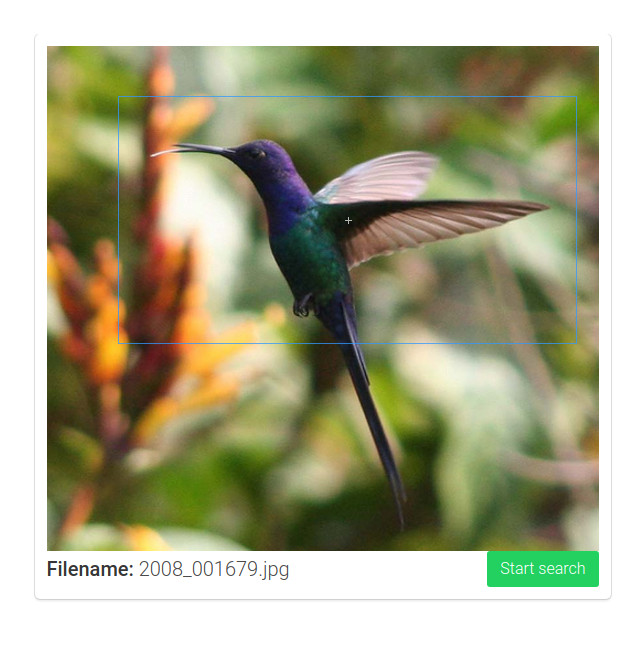
\includegraphics[height=4.5cm]{figures/server_select} &
        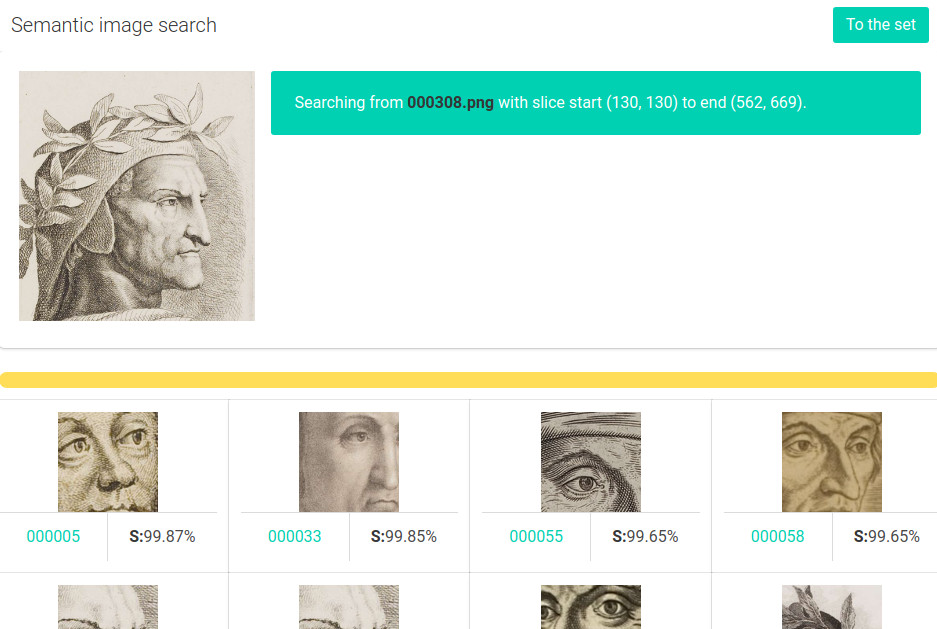
\includegraphics[height=4.5cm]{figures/server_results}
    \end{tabulary}
    \caption{Two screenshots of the provided online app using our method. Left shows the selection screen doing a new search. Right is the result screen displaying new finds.}
    \label{fig:application}
\end{figure}
We bring the described method to an application as a semantic image search machine. For this we build a small exemplar web application using the Flask microframework.

After configuring the program for a new image database the web application enables users to visually select a object or a part from one of the images of the set. The \gls{gui} provides a simple way to select a rectangular part of an image. Next the user can start the search with the selected patch. The backend quickly fine-tunes the \gls{resnet} under the same conditions as described in \treft{sec:results}.

Following the training the network is instantly reshaped into the \gls{fcn} and set up for normal image forwarding. The images from the database are all forwarded through the detection pipeline. In the meantime the collects the best results and presents the patches with the highest score to the user in descending order by their scores.
